\subsection{Analisi del problema}

Le problematiche emerse inizialmente dall'analisi dei requisiti e riguardanti i componenti sono:

\begin{enumerate}
\item  \textbf{distribuzione}: il robot e la console sono fisicamente in due posti diversi, quindi il sistema deve essere distribuito;
\item \textbf{eterogeneità}: il robot e la console potrebbero utilizzare tecnologie diverse, quindi il sistema deve essere eterogeneo;
\item \textbf{interazione}: trattandosi di un sistema distribuito eterogeneo, il sistema deve essere message-based e event-based per permettere alle entità di interagire tra di loro;
\item \textbf{coordinazione}: il robot e la console devono coordinarsi tra loro, quindi è opportuno stabilire una policy per definire quando e come determinate azioni devono verificarsi.
\end{enumerate}

Nella \cref{fig:system_external_view} è rappresentato il primo modello del sistema. In questo modello è possibile osservare che vi sono 3 entità: operatore, console e robot.

\begin{figure} [H]
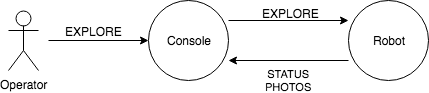
\includegraphics[width=\linewidth]{img/sprint0/system_external_view.png}
\caption{Il sistema osservato da un punto di vista esterno.}
\label{fig:system_external_view}
\end{figure}

Analizzando più nel dettaglio il problema sono emerse le seguenti problematiche: 
\begin{enumerate}
    \item \textbf{Come riceve i comandi la console?}\\
    In questo sistema, l'interazione tra l'operatore e la console può essere modellata a procedure call: l'operatore preme un pulsante su un'interfaccia grafica, la console elabora il comando verificando che esso sia valido e infine chiama la procedura adatta alla sua gestione. 
    Essendo tutto gestito internamente al componente console, risulta inutile utilizzare i paradigmi più complessi (ad esempio, message-based e event-based).
        
    \item \textbf{Come interagiscono console e robot?}\\
    Essendo un sistema distribuito la console e il robot interagiscono attraverso lo scambio di messaggi. I messaggi scambiati tra le due entità sono formalizzati di seguito.
    
       \begin{lstlisting}
//Message from console to robot
Dispatch explore: explore(X)
Dispatch stopExplore: stopExplore(X)
Dispatch backHome: backHome(X)
Dispatch continueExplore: continueExplore(X)
Dispatch backHomeSinceBomb: backHomeSinceBomb(X)
Dispatch continueExploreAfterPhoto: continueExploreAfterPhoto(X)

//Message from robot to console
Dispatch sendPhoto: sendPhoto(X)

//Message from robot to robot
Dispatch reachBag: reachBag(X)

    \end{lstlisting}
   
   \item \textbf{Quali informazioni bisogna mantenere sul modello del robot?}\\
   Il modello del robot può essere descritto attraverso un insieme di informazioni riguardanti:
   \begin{enumerate}
       \item lo stato (per sapere se il robot è fermo, sta andando avanti o indietro, si sta ruotando a destra o sinistra);
       \item la direzione (per sapere sapere come è orientato il robot all'interno della stanza: nord, sud, ovest, est);
       \item la posizione (per sapere dove si trova il robot all'interno della stanza).
   \end{enumerate} 
   
  In particolare, per rintracciare la posizione del robot all'interno della stanza, si utilizza il concetto di griglia, assumendo che esso si muova di passi unitari su di questa.
    
    \item \textbf{Come fa la console ad avere le informazioni riguardanti lo stato del robot?}\\
    Ogni volta che il robot cambia stato emette un evento con le informazioni aggiornate riguardanti il nuovo stato assunto. Tali informazioni verranno poi inviate alla console. L'evento emesso è formalizzato di seguito. 
    
    \begin{lstlisting}
Event modelContent: content(X)

\end{lstlisting}


Lo stato del robot è inizialmente modellato utilizzando Prolog come:

\begin{lstlisting}
//robot state formalisation
state(position(X,Y), direction(D), action(A))

position(X, Y)

direction(west)
direction(east)
direction(north)
direction(south)

action(moving)
action(stop)
action(take_picture)
action(send_photo)

\end{lstlisting}
        
    \item \textbf{Come viene percepito il cambiamento di temperatura della stanza?}\\
    Di default si assume che la temperatura della stanza sia inferiore ad una certa soglia finché al robot non arriva il messaggio di "temperatureTooHigh", il quale indica che la soglia è stata superata. I messaggi inviati al robot sono i seguenti:
   
    \begin{lstlisting}
Dispatch temperatureTooHigh: temperatureTooHigh
Dispatch temperatureOk: temperatureOk

\end{lstlisting}
        
    \item \textbf{Chi invia il messaggio della cambiamento della temperatura?}\\
    Ogni volta che la temperatura supera una certa soglia si scatena un evento che è percepito e gestito dalla console, la quale provvederà all'invio del messaggio "temperatureTooHigh" al robot.
        
    \item \textbf{Come fa il robot ad esplorare la stanza?}\\
     La stanza viene esplorata in maniera autonoma dal robot, quest'ultimo costruisce progressivamente una mappa della stanza riportando su di essa ostacoli fissi, ossia le valigie e i muri, con le relative posizioni e dimensioni. Questo compito può essere suddiviso in due fasi:  
    \begin{itemize}
        \item esplorazione della stanza vuota.
        \item esplorazione con ostacoli fissi.
    \end{itemize}{}
    
    \item \textbf{Quale strategia si può adottare per svolgere l'esplorazione della stanza vuota?}
    È possibile esplorare la stanza vuota in maniera incrementale: il robot coprirà dapprima una piccola area (a lui circostante) che mano a mano si espanderà fino a ricoprire l'intera stanza.
    
    \item \textbf{Quale strategia si può adottare per svolgere l'esplorazione della stanza con ostacoli fissi?}
    È possibile esplorare la stanza con ostacoli fissi in maniera simile a quanto accadrebbe nel caso in cui la stanza fosse vuota: il robot, partendo dalla sua posizione iniziale, esplorerà dapprima la parte di stanza più vicina a lui per poi successivamente espandersi sempre di più. Ogni qual volta il robot si trovi in presenza di un ostacolo, si ricalcolerà un percorso per raggiungere la posizione desiderata sulla griglia. Inoltre, verranno memorizzate le informazioni relative all'ostacolo.
    
    \item \textbf{Come fa il robot a riconoscere un ostacolo?}\\
    Assumiamo che il robot sia dotato nella parte frontale di un sonar e che ogni volta che il sonar rilevi un valore inferiore ad una certa soglia il robot si fermi in quanto si è in presenza di un ostacolo. 
    
    \item \textbf{Da quale prospettiva il robot scatta la foto all'ostacolo?}\\
    Il robot scatta la foto alla valigia esattamente dall'angolazione in cui esso si trova rispetto all'ostacolo nel momento in cui giunge in sua prossimità. Infatti, l'angolazione della foto risulta ininfluente ai fini della valutazione della presenza o meno della bomba, poiché si suppone che il tool utilizzato dalla console esamini il bagaglio con una tecnologia a infrarossi.
    
    \item \textbf{Come fa il robot a tornare nella posizione iniziale?}\\
    La prima cella , ossia (0,0), che il robot memorizza sulla mappa è la sua posizione iniziale, quindi basterà che esso percorra un qualunque tragitto dalla sua posizione attuale alla prima cella memorizzata della mappa per far sì che torni nella sua posizione iniziale.
    
    \item \textbf{In caso di valigia sospetta, cosa fa il robot?}\\
    La valigia sospetta sarà l'ultimo ostacolo memorizzato nella mappa, in quanto quando questo viene rilevato la fase di esplorazione si sospende. 
    Una volta individuata la valigia sospetta, il robot rientrà autonomamente alla base (R-backHomeSinceBomb) al robot. Quando quest'ultimo è tornato alla base (R-waitForHome), esso ripartirà per raggiungere la valigia sospetta, ossia l'ultima memorizzata sulla mappa (R-ReachBag), la inserirà poi in un contenitore e la trasporterà nella sua posizione iniziale (R-bagAtHome). 
    
    \item \textbf{Come fa la console ad interagire con il robot durante la fase di esplorazione?}\\
    Il robot dovrà avere una natura proattiva per gestire autonomamente l'esplorazione della hall e un natura reattiva per ricevere e rispondere prontamente ai messaggi della console.
    
\end{enumerate}

In base all'analisi del problema, si è derivata l'architettura logica di figura \ref{fig:arch_logica}. Al di sopra della linea sono rappresentate le entità principali che compongono il sistema e come queste interagiscono tra di loro , invece, al di sotto delle linea si trovano le relative implementazioni di tali entità.

\begin{figure}  [H]
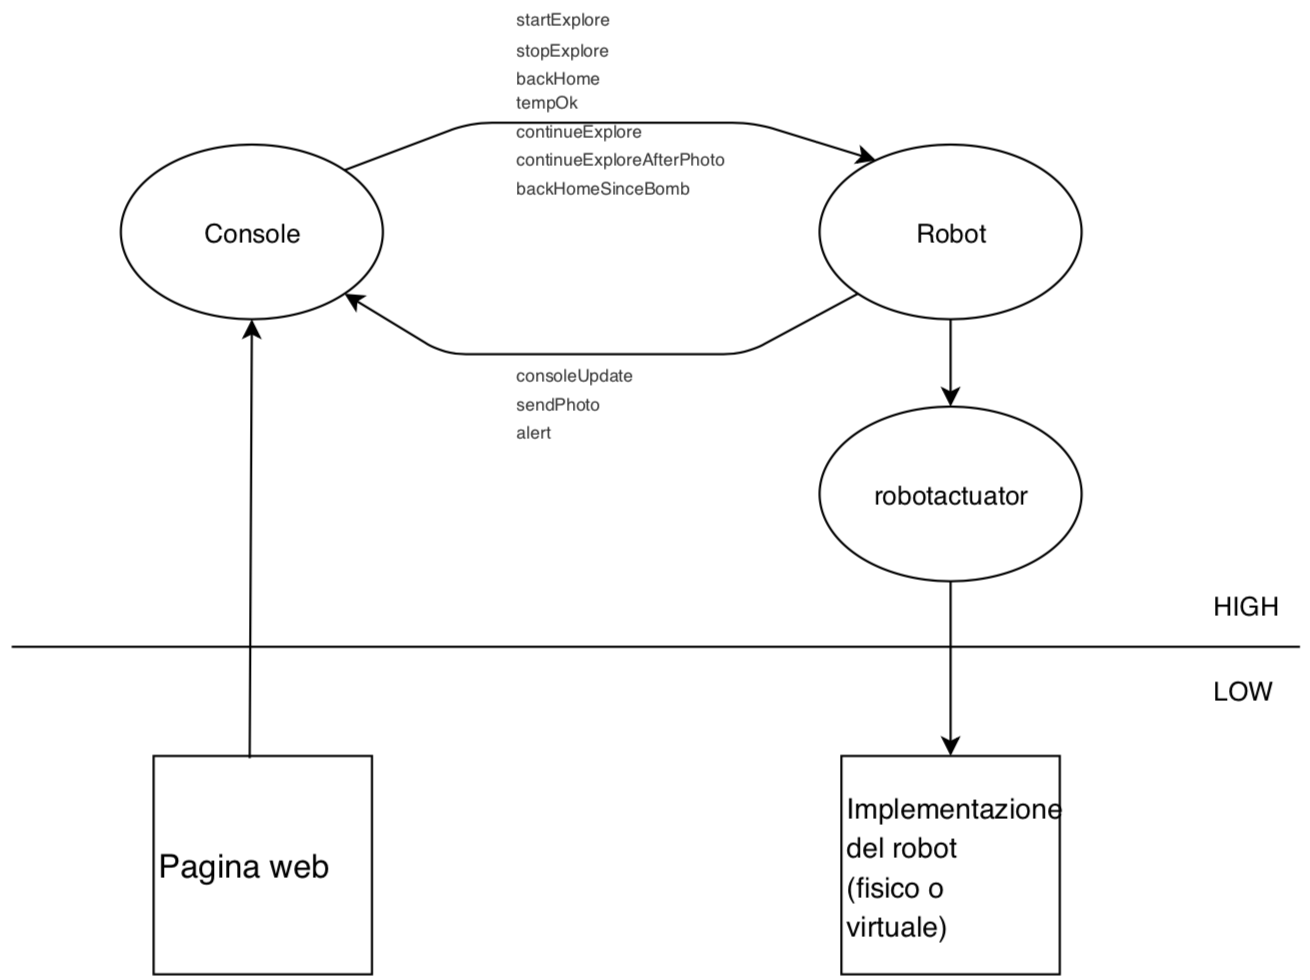
\includegraphics[width=\linewidth]{img/sprint0/arch_logica.png}
\caption{L'architettura logica del sistema.}
\label{fig:arch_logica}
\end{figure}


\subsection{Test Plan}
Nel Test Plan bisogna verificare che:
\begin{itemize}

    \item quando l'utente spinge il pulsante di startExploration e la temperatura della stanza è inferiore ad una soglia fissata, il robot inizi l'esplorazione.
    
     \item quando la console percepisce l'evento del cambio di temperatura, verifica se è ancora adeguata e se è troppo alta invia al robot il messaggio di stopExplore
    
    \item quando il robot riceve il messaggio di explore inizia ad esplorare tutta la stanza;
    
    \item quando il robot riceve il messaggio di stopExplore si ferma nel punto in cui si trova;
     
    \item quando il robot riceve il messaggio di backHome torna nella sua posizione iniziale;
    
    \item quando il robot incontra una valigia non ancora analizzata si ferma, gli scatta una foto e la spedisce con un messaggio alla console (sendPhoto). 
    
    \item quando il robot riceve il messaggio di continueExplore riprende l'esplorazione.
    
    \item quando il robot riceve il messaggio di comeBackSinceBomb torna alla base e passa alla fase di recupero della valigia pericolosa.
    
 
\end{itemize}







    
\begin{lstlisting}
System ddrSys

//robot state update event
Event consoleUpdate: consoleUpdate(X)

//temperature change event
Event tempOk: tempOk(X)

//Message from console to robot
Dispatch explore: explore(X)
Dispatch stopExplore: stopExplore(X)
Dispatch backHome: backHome(X)
Dispatch continueExplore: continueExplore(X)
Dispatch backHomeSinceBomb: backHomeSinceBomb(X)
Dispatch continueExploreAfterPhoto: continueExploreAfterPhoto(X)

//Message from robot to console
Dispatch sendPhoto: sendPhoto(X)

//Message from robot to robot
Dispatch reachBag: reachBag(X)


Context ctx ip [host="localhost" port=8078] -g cyan

QActor console context ctx { 
	
	Plan init normal [
		println("Console intialized")
	]
}

QActor robot context ctx { 
	Plan init normal [
		
		println("Robot intialized")
	]
} 
\end{lstlisting}

